
%\documentclass[mathserif]{beamer}
\documentclass[handout]{beamer}
\usetheme{Goettingen}
%\usetheme{Warsaw}
%\usetheme{Singapore}



%\usetheme{Frankfurt}
%\usetheme{Copenhagen}
%\usetheme{Szeged}
%\usetheme{Montpellier}
%\usetheme{CambridgeUS}
%\usecolortheme{}
%\setbeamercovered{transparent}
\usepackage[english, activeacute]{babel}
\usepackage[utf8]{inputenc}
\usepackage{amsmath, amssymb}
\usepackage[lined]{algorithm2e}


\usepackage{dsfont}
\usepackage{graphics}
\usepackage{cases}
\usepackage{graphicx}
\usepackage{pgf}
\usepackage{epsfig}
\usepackage{multirow}	
\usepackage{amstext}
%\usepackage[ruled,vlined,lined]{algorithm2e}
\usepackage{epic}
\usepackage{epsfig}
\usepackage{fontenc}
\usepackage{framed,color}
\usepackage{palatino, url, multicol}
%\algsetup{indent=2em}
\newcommand{\factorial}{\ensuremath{\mbox{\sc Factorial}}}
\newcommand{\BIGOP}[1]{\mathop{\mathchoice%
{\raise-0.22em\hbox{\huge $#1$}}%
{\raise-0.05em\hbox{\Large $#1$}}{\hbox{\large $#1$}}{#1}}}
\newcommand{\bigtimes}{\BIGOP{\times}}
\vspace{-0.5cm}
\title{Tackling Fairness, Change and Polysemy in Word Embeddings}
\vspace{-0.5cm}
\author[Felipe Bravo Márquez]{\footnotesize
%\author{\footnotesize  
 \textcolor[rgb]{0.00,0.00,1.00}{Felipe Bravo-Marquez}} 
  
 
%\vspace{-0.3cm}
\institute{Department of Computer Science, University of Chile \\ National Center for Artificial Intelligence Research \\ Millenium Institute Foundational Research on Data }

\titlegraphic{
\includegraphics[scale=0.06]{pics/logodcc.png}
\includegraphics[scale=0.02]{pics/cenialogo.jpg} 
\includegraphics[scale=0.4]{pics/imfdlogo.png}
\includegraphics[scale=0.15]{pics/RELELA.png}}



\date{\today}

\begin{document}
\begin{frame}
\titlepage


\end{frame}

\section{Introduction}

\begin{frame}{Word Embeddings}
\begin{scriptsize}
\begin{itemize}
\item The first step in computationally working with written language is to represent words as mathematical objects  we can operate with.

\item Representing words as numeric vectors a.k.a \textbf{embeddings} is a standard practice in \textbf{Natural Language Processing} (NLP).

\item Word embeddings are a mapping of discrete symbols (i.e., words) to continuous vectors.


\item Distance between vectors can be equated to distance between words.
\item This makes easier to generalize the behavior from one word to another.

\item Word embeddings have become a \textbf{core component} of NLP downstream systems (e.g., sentiment analysis, machine translation, question answering).


\end{itemize}
\end{scriptsize}
\end{frame}


\begin{frame}{Word Embeddings}
\begin{figure}[h]
  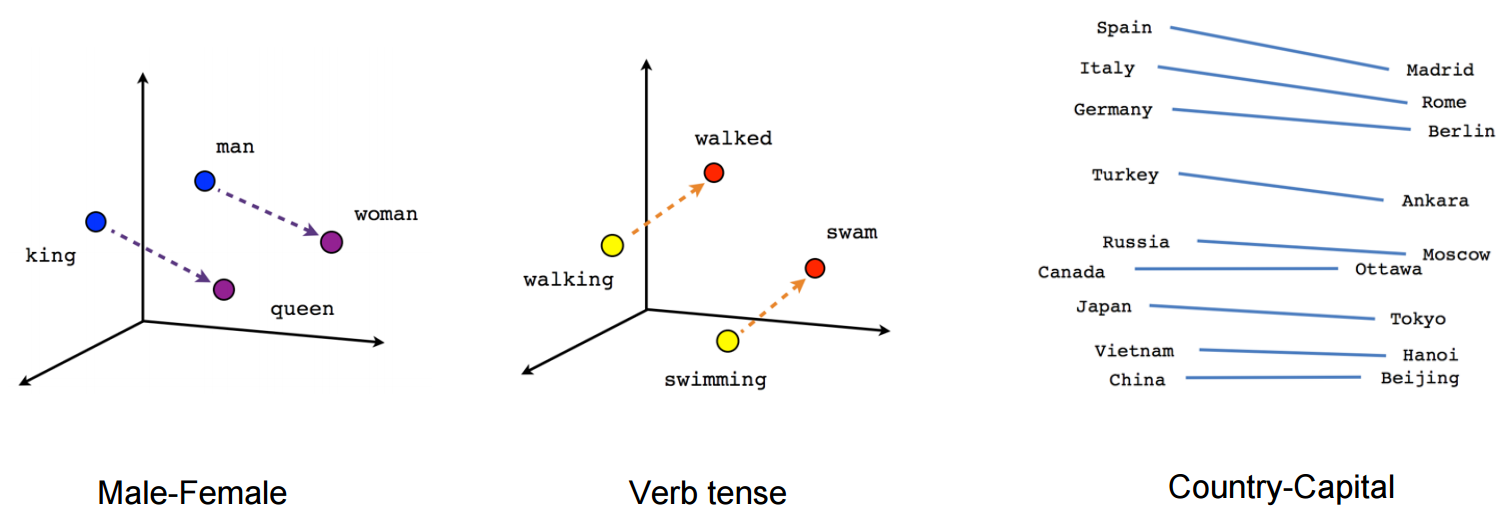
\includegraphics[scale=0.17]{pics/embeddings.png}
\end{figure}
Word embeddings can encode semantic and syntatic relationships between words.


\end{frame}




\begin{frame}{Distributional Hypothesis}
\begin{scriptsize}
\begin{itemize}
\item The construction of word embeddings from document corpora is based on the  \textbf{Distributional Hypothesis} \cite{harris1954}:
\begin{quote}
 Words occurring in the same \textbf{contexts} tend to have similar meanings.
\end{quote}

\item Or equivalently:
\begin{quote}
A word is characterized by the \textbf{company} it keeps.
\end{quote}


\item The idea is to map words occuring in similar contexts to similar vectors.

\end{itemize}
\end{scriptsize}
\end{frame}


\begin{frame}{Word Embeddings}
\begin{figure}[h]
  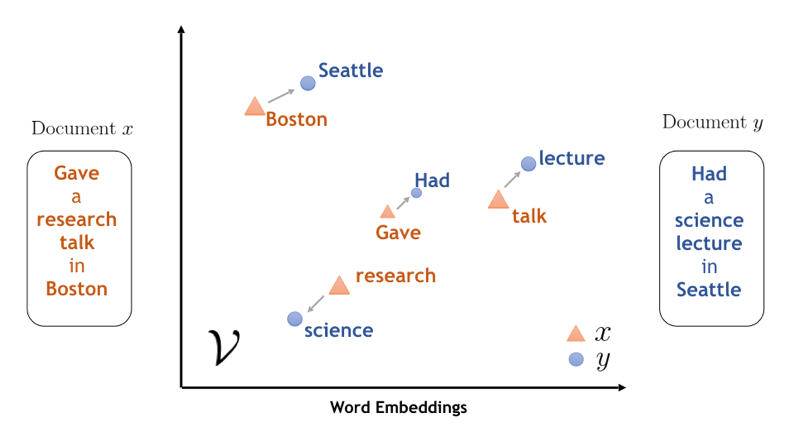
\includegraphics[scale=0.7]{pics/embeddings2.png}
\end{figure}



\end{frame}



\begin{frame}{Word Embeddings Algorithms}
\begin{scriptsize}
\begin{itemize}
\item Word embeddings are build by training \textbf{neural networks} architectures on document \textbf{corpora} (e.g., books, papers, Wikipedia, tweets, the Web).

\item These arquitectures formulate a \textbf{predictive task} (e.g., predict a missing word withing a contex window) in which word embeddings naturally arise from the network's parameters after training.

\item Most popular models are:
\begin{itemize}
\scriptsize{
\item Skip-gram negative sampling \cite{Mikolov2013}
\item Continuous bag-of-words \cite{Mikolov2013}
\item Glove \cite{penningtonSM14}
\item FastText \cite{bojanowski2016enriching}.}
\end{itemize}




\end{itemize}
\end{scriptsize}
\end{frame}

\begin{frame}{Skip-gram Model}

  \begin{figure}[h]
        	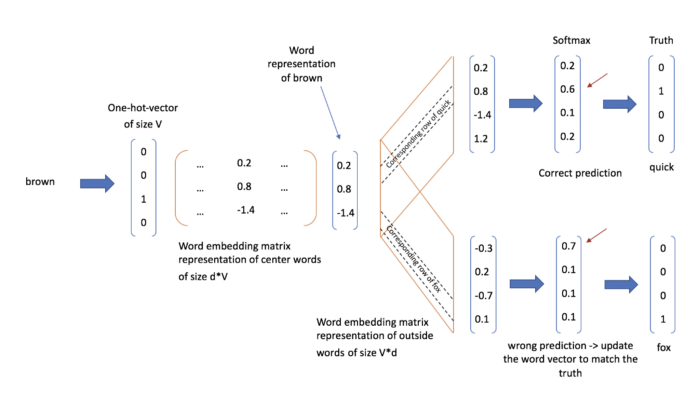
\includegraphics[scale = 0.4]{pics/skip_gram_net_arch.png}
        \end{figure}
\footnotetext{Picture taken from:    \url{http://mccormickml.com/2016/04/19/word2vec-tutorial-the-skip-gram-model/}}

\end{frame}


\begin{frame}{Limitations of Word Embeddings}
\begin{scriptsize}
\begin{itemize}


\item In this talk we will present our research addressing three limitations of word embeddings.

\begin{enumerate} \scriptsize{
 \item \textbf{Fairness}: they are prone to inherit stereotypical social biases from the corpus they were built on.
 \item \textbf{Change}: they are static. Thus they ignore words not observed during training and are unable to capture semantic drifts.
 \item \textbf{Polysemy}: they fail to capture the polysemous nature of many words (e.g., apple:company, apple:fruit), conflating their multiple senses into a single point.
}
\end{enumerate}




\end{itemize}
\end{scriptsize}
\end{frame}

\section{Fairness}


\begin{frame}{Fairness in Word Embeddings}
\begin{scriptsize}
 Word Embeddings have showed to exhibit undesireded associations between words for certain social groups (e.g., gender, race, religion):
\begin{itemize}
\item Black is to criminal as caucasian is to police.
\item Man is to doctor as woman is to nurse.
\item Man is to computer programmer as woman is to homemaker.
\end{itemize}


\end{scriptsize}
\end{frame}

\begin{frame}{Fairness Metrics}
\begin{scriptsize}

\begin{itemize}
 \item \textbf{WEAT} \cite{caliskan2017semantics}:  Degree of association between two sets of target words and two sets of attribute words.

 \begin{itemize}\scriptsize{
 \item Studies biases regarding ethnicity (in relation to pleasant-unpleasant words) and gender (in relation to occupations).}
 \end{itemize}

\item \textbf{RND} \cite{garg2018word}: Compares the embeddings related to two different social group against a set of neutral words.
 \begin{itemize}\scriptsize{
 \item Embeddings trained on different periods of time were evaluated to test to gender and ethnic biases. }
 \end{itemize}

\item \textbf{RNSB} \cite{sweeney2019transparent}:  KL divergence between the negative sentiment probability of the embeddings and a uniform distribution.
 \begin{itemize}\scriptsize{
 \item Test a set of national origin identity terms such as American, Mexican, and Canadian. }
 \end{itemize}
\end{itemize}






\end{scriptsize}
\end{frame}


\begin{frame}{WEFE: The Word Embeddings Fairness Evaluation Framework}
\begin{scriptsize}
\begin{itemize}
\item Although metrics have similar objectives they cannot be easily compared with each other.
\item They operate with different inputs (e.g., pairs of words, sets of words, multiple sets of words).
\item Their outputs are also incompatible with each other (e.g., reals, positive numbers, $[0,1]$ range).
 \item The \textbf{Word Embeddings Fairness Evaluation (WEFE)} is a framework for measuring and mitigating bias in word embeddings \cite{badilla2020wefe}.

 \item  WEFE formalizes existing fairness metrics into a \textbf{unified framework}.
\end{itemize}

\end{scriptsize}
\end{frame}


\begin{frame}{WEFE: The Word Embeddings Fairness Evaluation Framework}
\begin{scriptsize}
\begin{itemize}

 \item It encapsulates the input words of these metrics into standard objects called \textbf{queries}.
 \item Then, proceeds to quantify the bias of word embeddings using these queries along with different fairness metrics.
 \item It also allows for \textbf{ranking} multiple embeddings models by aggregating the previous scores.
\end{itemize}
  \begin{figure}[h]
        	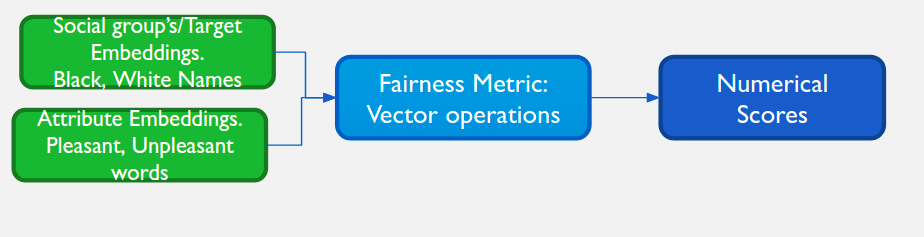
\includegraphics[scale = 0.3]{pics/wefe.png}
        \end{figure}

\end{scriptsize}
\end{frame}

\begin{frame}{WEFE Building Blocks}
\begin{scriptsize}
\begin{itemize}

 \item \textbf{Target Sets}:  a set of words intended to denote a particular social group. \\ For example:


   \begin{align}
T_{\text{women}}  =  \{w_{\text{she}},w_{\text{woman}},w_{\text{girl}}, \ldots\}, \\
T_{\text{men}}  =  \{w_{\text{he}},w_{\text{man}},w_{\text{boy}}, \ldots\},
 \end{align}


 \item \textbf{Attribute Sets}: a set of words representing some attitude, characteristic, trait, occupational field, etc. that can be associated with individuals from any social group. \\ For example:

    \begin{align}
 A_{\text{science}} =  \{w_{\text{math}},w_{\text{physics}},w_{\text{chemistry}}, \ldots\}, \\
A_{\text{art}} = \{w_{\text{poetry}},w_{\text{dance}},w_{\text{literature}}, \ldots\}.
 \end{align}


  \item \textbf{Query}: a pair $Q=(\mathcal{T},\mathcal{A})$ in which $\mathcal{T}$ is a set of target word sets, and $\mathcal{A}$ is a set of attribute word sets. \\ For example:

 \begin{equation}\label{eq:query}
Q=(\{T_{\text{women}}, T_{\text{men}}\},\{A_{\text{science}},A_{\text{art}}\}).
\end{equation}

 \end{itemize}


\end{scriptsize}
\end{frame}

\begin{frame}{WEFE Building Blocks}
\begin{scriptsize}
\begin{itemize}

\item Queries are the main building blocks used by fairness metrics to measure bias of word embedding models.

\item Fairness metrics encapsulated by WEFE are defined with a query template $s_F=(t,a)$, which is a pair of natural values  with the cardinalities of sets $\mathcal{T}$ and $\mathcal{A}$.

\item We equip each metric with a total order relation $\leq_F$ that establishes what is to be considered as \emph{less biased}.


\item That is, if
\begin{displaymath}
 F(\mathbf{M_1},Q)\leq_F F(\mathbf{M_2},Q)
\end{displaymath}
we can say that \emph{$\mathbf{M_1}$ is less biased than model $\mathbf{M_2}$}.

\item With this order relation we can rank various embeddings models according to their biases.

 \end{itemize}


\end{scriptsize}
\end{frame}


\begin{frame}{WEFE Toolkit}
\scriptsize{We released WEFE as an open source Python software:
\url{https://wefe.readthedocs.io/}

  \begin{figure}[h]
        	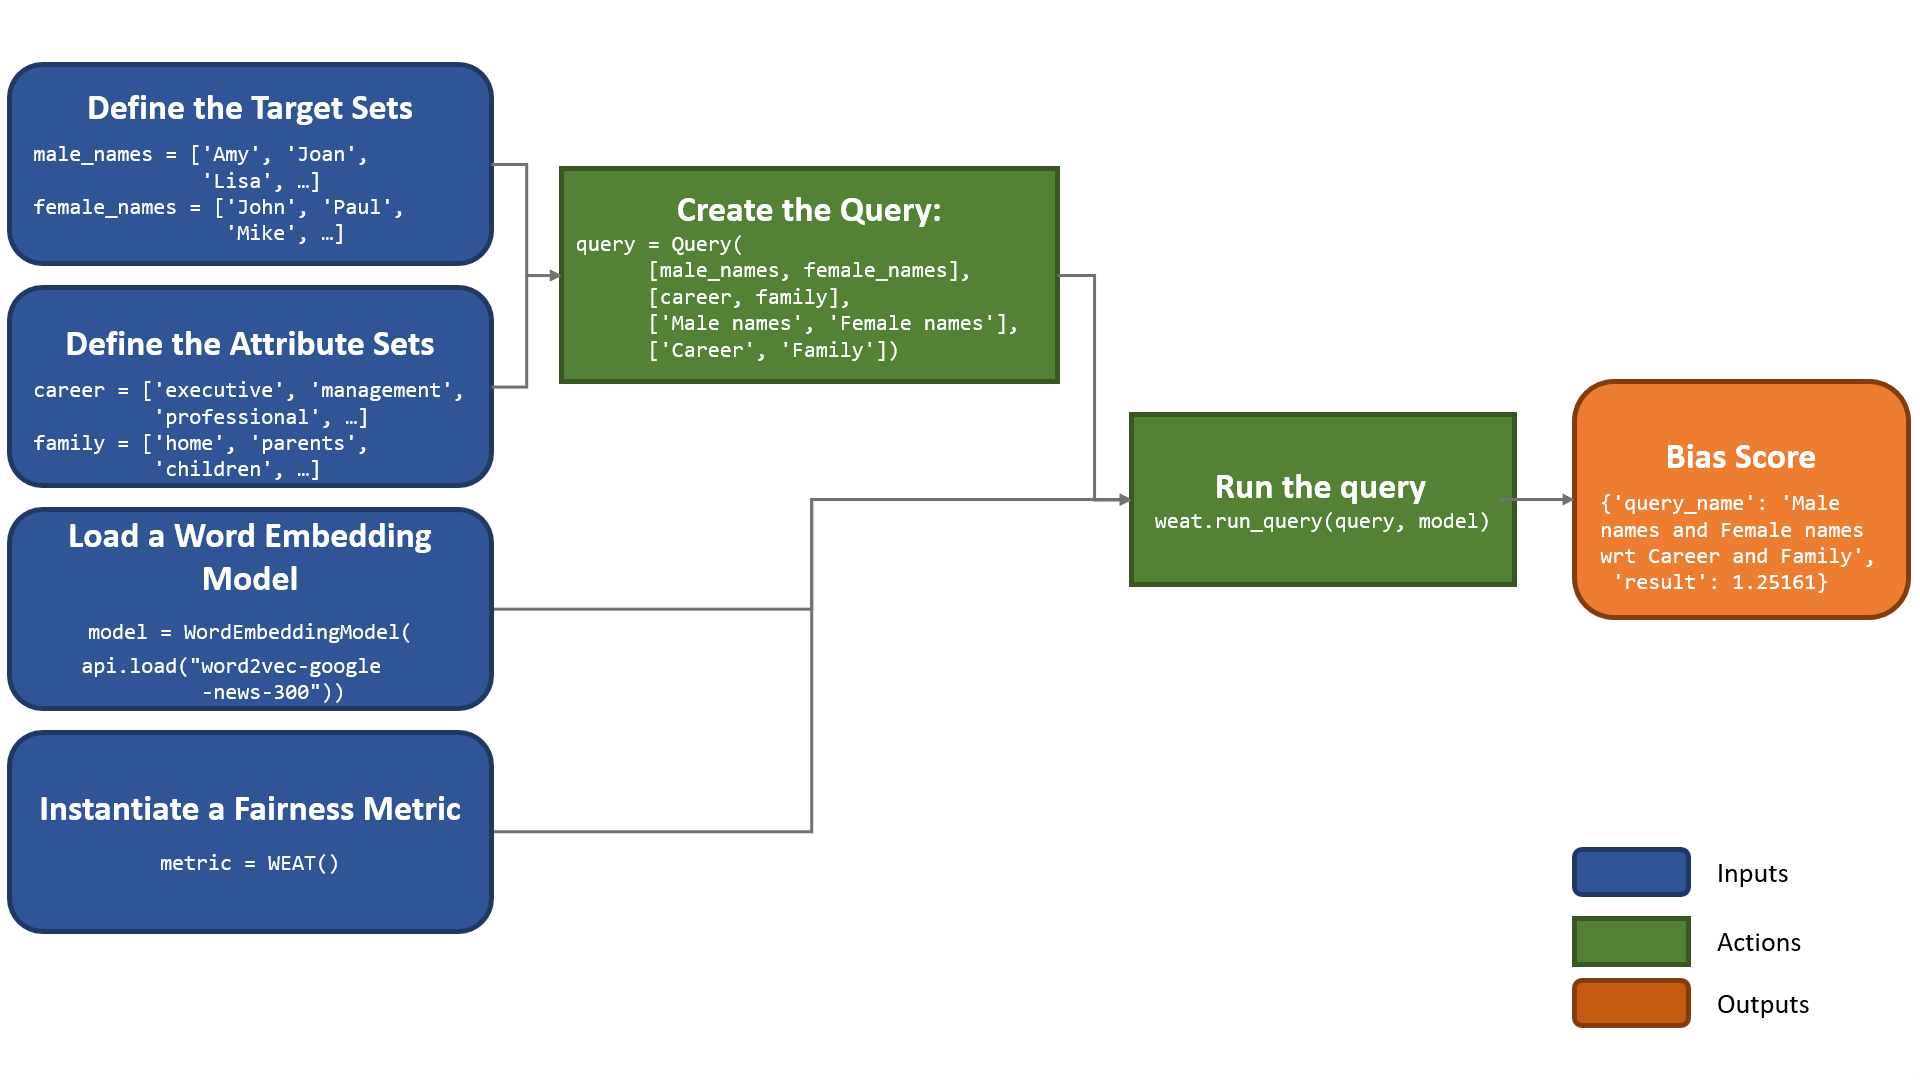
\includegraphics[scale = 0.22]{pics/wefedia.png}
        \end{figure}


        }

\end{frame}

\begin{frame}{Case Study}
\scriptsize{
We used WEFE to rank various embedding models according to their aggregated biased with respect to to gender, religion and ethnicity:}


  \begin{figure}[h]
        	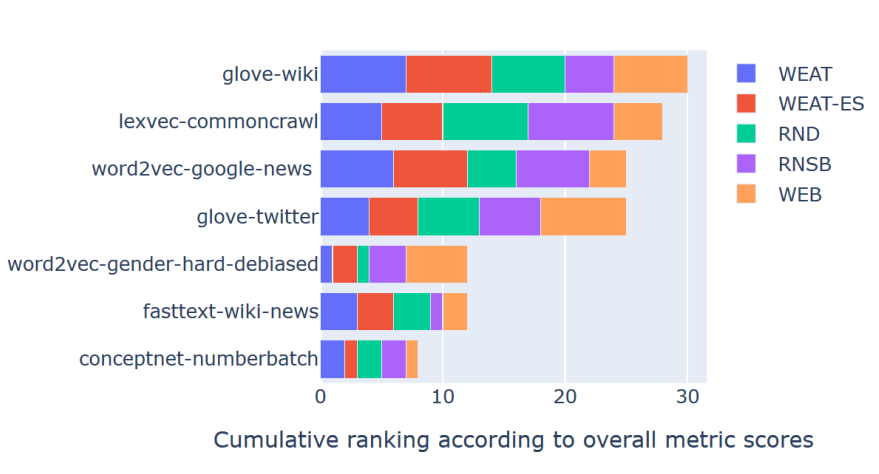
\includegraphics[scale = 0.3]{pics/weferanking.png}
        \end{figure}

\end{frame}


\section{Change}

\begin{frame}{Incremental Word Vectors for time-evolving sentiment lexicon induction}
\begin{scriptsize}
\begin{itemize}
 \item  A sentiment lexicon is a list of expressions annotated according to affect categories such as positive, negative, anger and fear.

 \item  Lexicons are widely used in sentiment classification of tweets.

 \item They are usually build by training a word-level sentiment classifier on pre-trained word embeddings using a \textbf{seed lexicon} as training data \cite{TangCol14}.

 \item  However, as word embeddings are static by nature, sentiment lexicons build in this way are  unable to capture:

 \begin{enumerate} \scriptsize{
  \item The arrival of new sentiment-conveying expressions such as \#trumpwall and \#PrayForParis.
  \item Temporal changes in sentiment patterns of words (e.g., a scandal associated with an entity).}
 \end{enumerate}



\end{itemize}


\end{scriptsize}
\end{frame}


\begin{frame}{Incremental Word Vectors for time-evolving sentiment lexicon induction}
\begin{scriptsize}

 We developed a methodology for automatically inducing \textbf{continuously updated} sentiment lexicons from \textbf{Twitter streams} by training \textbf{incremental} word sentiment classifiers from \textbf{time-evolving word vectors}. \cite{bravo2021incremental}
  \begin{figure}[h]
        	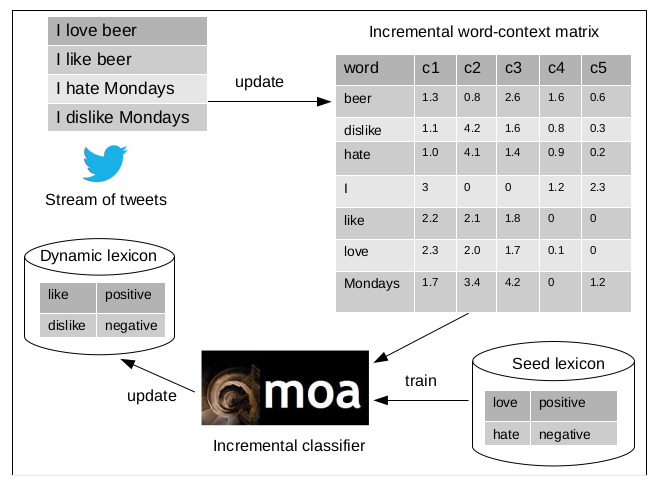
\includegraphics[scale = 0.35]{pics/incdiagram.png}
        \end{figure}

\end{scriptsize}
\end{frame}

\begin{frame}{Incremental Word Vectors for time-evolving sentiment lexicon induction}
\begin{scriptsize}

 The process is summarized as follows:

 \begin{enumerate}
    \item Connect to a stream of continuously arriving text (e.g., Twitter).
    \item Every time a new tweet arrives, a sliding window of $W$ words centered on a target word is shifted across the content.
    \item The word vector associated with the target word is updated according to its context. This process implies updating  word-context counts and computing PPMI-based associations.
    \item If the target word is new, a new vector associated with this word is created.
    \item If the target word is contained in the seed lexicon, the incremental classifier is updated/trained using the target word vector and the lexicon's sentiment as the gold label.
    \item If the target word is not contained in the lexicon, its sentiment is estimated using the classifier and the dynamic lexicon is updated.
\end{enumerate}


\end{scriptsize}
\end{frame}


\begin{frame}{Incremental Algorithms}

\scalebox{.5}{
\begin{algorithm}[H]

  \KwData{tweets, window size $W$, vocabulary size $V$, context size $C$}
  \KwResult{PPMI Matrix $M$}
    Initialize PPMI Matrix $M$ of size $V \times C$\;
    $D$ $\leftarrow$ 0\;
    \While{tweet in Data Stream}{
       tokens $\leftarrow$ tokenize(tweet)\;
      \For{\textbf{each} $w$ in tokens}{
       $D$ $\leftarrow$ $D+1$\;
       $c_1, \dots, c_{2W}$ $\leftarrow$ getContexts($w$,tokens)\;
       updateContextMatrix($w,c_1, \dots, c_{2W}$)\;
       \For{\textbf{each} $c_j$ in $c_1, \dots, c_{2W}$}{
        PPMI$(w,c_j)$ $\leftarrow$  $\max \left (0, \log_{2} \left ( \frac{count(w,c_j)\times D}{count(w)\times count(c_j)} \right ) \right )$ \;
       %$PPMI^{w}_{0 \dots C}$ $\leftarrow$ PPMI($w$,$c_{0 \dots W}$,$|D|$)
       }
      }
    }

\end{algorithm}}

\scalebox{.5}{
\begin{algorithm}[H]
    \KwData{tweets, training seed lexicon, testing seed lexicon}
    \While{Tweet $T$ in Data Stream}{
        % tokens $\leftarrow$ tokenize($T$)\;
        \For{\textbf{each} token t in tokens}{
            updateContextCounters($t$,$T$)\;
            updatePPMIValues($t$,$T$)\;
            \uIf{token $\in$ train seed lexicon}{
               trainClassifier(PPMI($t$),label($t$))\;
            }
            \uElseIf{token $\in$ test seed lexicon}{
                updateEvaluator(PPMI($t$),label($t$))\;
            }
        }
    }
\end{algorithm}}

\end{frame}




\begin{frame}{Sentiment Drifts}
\begin{scriptsize}
\begin{itemize}
 \item We simulate sentiment change by randomly picking some words and swapping their context with the context of words exhibiting the opposite sentiment.

   \begin{figure}[h]
        	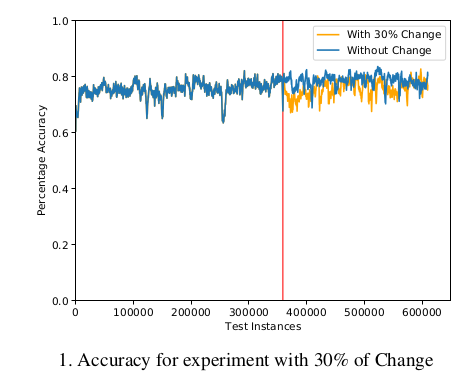
\includegraphics[scale = 0.25]{pics/change1.png}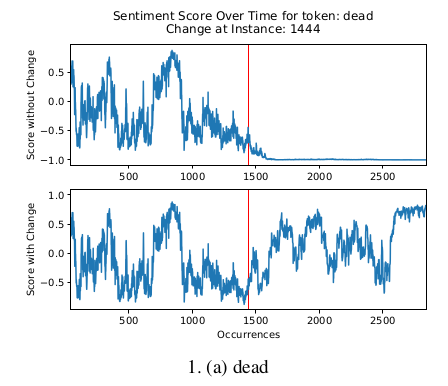
\includegraphics[scale = 0.3]{pics/change.png}
        \end{figure}

 \item Our approach allows for successfully tracking of the sentiment of words over time even when drastic change is induced.

\end{itemize}


\end{scriptsize}
\end{frame}




\section{Polysemy}

\begin{frame}{PolyLM: a polysemous language model}
\begin{scriptsize}
\begin{itemize}
 \item PolyLM is a language model capable of automatically learning multiple meanings of a word (e.g. apple:apple, apple:company) \cite{ansell2021polylm}.

   \begin{figure}[h]
        	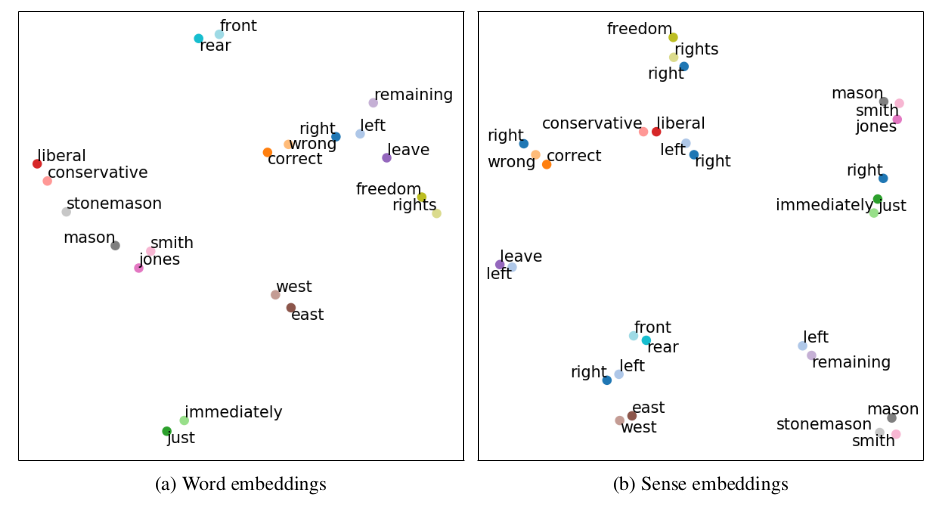
\includegraphics[scale = 0.25]{pics/senseembeddings.png}
        \end{figure}


   \item  The occurrence of closely related polysemous words nearby in the word embedding space (i.e. \textit{left} and \textit{right}) causes unrelated words to be closer together (e.g. \textit{left} and \textit{wrong}) and related words to be further apart (e.g. \textit{right} and \textit{east}) than they otherwise would be


\end{itemize}



\end{scriptsize}
\end{frame}


\begin{frame}{PolyLM: a polysemous language model}
\begin{scriptsize}
\begin{itemize}
 \item PolyLM is an unsupervised language model based on two assumptions:

 \begin{enumerate}\scriptsize{
  \item The probability of a word occurring in a given context is equal to the sum of the probabilities of its individual senses.
  \begin{align}
    p(w | c) = \sum_{s \in S_w} p(s | c).
\end{align}

  \item For a given occurrence of a word, one of its senses tends to be much more plausible in the context than the others.
  }
 \end{enumerate}

\item PolyLM is based on a Transformer encoder architecture and the masked language modeling (MLM) task used for training BERT.

\item Its loss function  combines a standard  language modeling loss with a distinctness loss  encouraging one sense to have a high estimated probability of occurring, and the rest to have a low probability.





 \end{itemize}
\end{scriptsize}
\end{frame}




\begin{frame}{PolyLM: a polysemous language model}

  \begin{figure}[h]
        	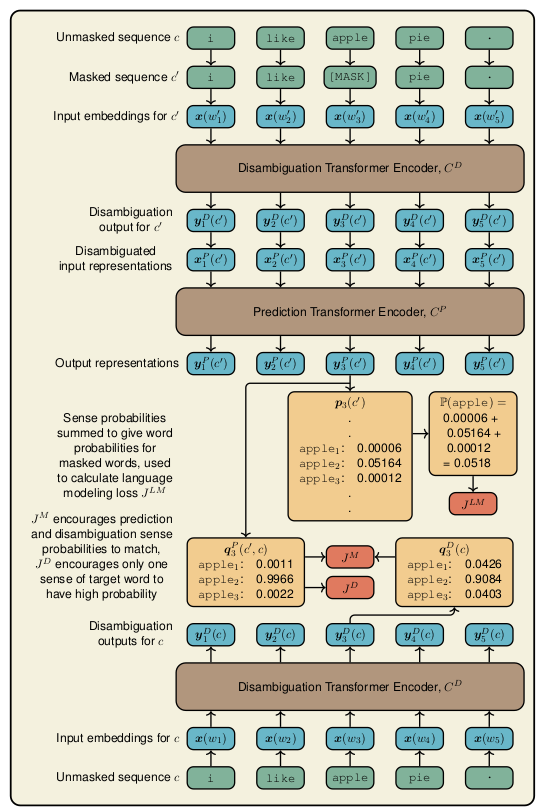
\includegraphics[scale = 0.29]{pics/polylm.png}
        \end{figure}


\end{frame}



\begin{frame}{Results on the Word Sense Induction (WSI) task}
\begin{scriptsize}
\begin{table}
    \centering
    \resizebox{\textwidth}{!}{\begin{tabular}{llcccccc}
               \hline
        \multirow{2}{*}{\textbf{System}} & \multirow{2}{*}{\textbf{Version}} & \multicolumn{3}{c}{\textbf{SemEval-2010}} & \multicolumn{3}{c}{\textbf{SemEval-2013}} \\
        && F-S & V-M & \textbf{AVG} & FBC & FNMI & \textbf{AVG}\\
        \hline
        Aamrami-goldberg& BERT$_\text{LARGE}$ & \textbf{71.3} & 40.4 & \textbf{53.6} & 64.0 & 21.4 & 37.0\\
        AutoSense & & 62.9 & 10.1 & 25.2 & 61.7 & 8.0 & 22.2\\
        \hline
        \multirow{2}{*}{PolyLM$^{\dagger}$} & BASE & 65.8 & \textbf{40.5} & 51.6 & \textbf{64.8} & \textbf{23.0} & \textbf{38.6}\\
        & SMALL & 65.6 & 35.7 & 48.4 & 64.5 & 18.5 & 34.5\\
        \hline
        Qiu et. al$^\dagger$ & & - & - & - & 56.9 & 6.7 & 19.5\\
        SE-WSI-fix-cmp$^\dagger$ & & 54.3 & 16.3 & 29.8 & - & - & -\\
        AdaGram$^\dagger$ & & 43.9 & 20.0 & 29.6 & 13.2 & 8.9 & 10.8\\
        Arora et. al$^\dagger$ & $k = 5$ & 46.4 & 11.5 & 23.1 & - & - & -\\
        \hline
    \end{tabular}}
    \caption{Comparison of sense embedding models and WSI-specific techniques on the SemEval 2010 and 2013 WSI tasks. SE-WSI-fix-cmp is based on MSSG model. $^\dagger$ - models which obtain explicit sense embeddings.}
    \label{tab:wsi}
\end{table}
\end{scriptsize}
\end{frame}


\begin{frame}{Conclusions}

\begin{itemize}
\item In this talk we have presented three research projects, each addressing a different limitation of word embeddings.


\item I would like to thank all the co-authors of the presented works: Alan, Arun, Jorge, Pablo and Bernhard.

\item There is plenty of room for further research.
\end{itemize}


\end{frame}


\begin{frame}
\frametitle{Questions?}
%\vspace{1.5cm}
\begin{center}\LARGE Thanks for your Attention!\\ \end{center}



\end{frame}

\begin{frame}[allowframebreaks]\scriptsize
\frametitle{References}
\bibliography{bio}
\bibliographystyle{apalike}
%\bibliographystyle{flexbib}
\end{frame}  


%%%%%%%%%%%%%%%%%%%%%%%%%%%

\end{document}
